% \subsection{OpenTelemetry}
% \label{subsec:opentelemetry}

Es haben sich auf Basis dieser drei Grundpfeiler einige Technologien entwickelt. Jedoch sind die meisten Ansätze proprietär und nicht miteinander kompatibel, weswegen das Bedürfnis einer Standardisierung entstand. OpenTracing, OpenCensus \cite{OpenCensus} sowie OpenTelemetry \cite{OpenTelemetry} sind aus dieser Bewegung stammende Standards, die darauf abzielen herstellerunabhängige Observability-Konzepte zu definieren.

OpenTelemetry (OTel) ist ein sich derzeit\footnote{Ein erster (General-Availability-)Release der Spezifikation ist für die erste Hälfte 2021 geplant \cite{OpenTelemetryGARelease}.} entwickelnder Standard, welcher als Ziel hat, dass das erfassen, weiterleiten und verarbeiten von  Tracing-, Metrik- und Logdaten\footnotemark{} herstellerunabhängig ermöglicht wird. OTel entwickelte sich aus dem Zusammenschluss der Teams hinter den beiden Standards OpenTracing und OpenCensus, die das gleiche Ziel der Vereinheitlichung, der hier existierenden Ansätze, verfolgen  \cite{UseNixDistributiveTracing}. Weiterhin versucht OTel nicht nur die bisherige Landschaft zu vereinigen, sondern definiert bspw. eine zukunftsorientierte Architektur aus unterschiedlichen Komponenten und wie diese miteinander kommunizieren \cite{DistributedTracingInPractice}. Microsoft, Google, die Cloud-Native-Computing-Foundation (CNCF) sowie führende Unternehmen und Entwickler von Observability-Technologien arbeiten an der Voranschreite des OTel Standards \cite{DistributedTracingInPractice} \cite{OpenTelemetryCommunityMembers}.

\nomenclature[Fachbegriff]{OTel}{OpenTelemetry}
\nomenclature[Fachbegriff]{CNCF}{Cloud-Native-Computing-Foundation}
\footnotetext{Die Entwicklung einer Logging-Spezifikation ist im Gange \cite{OpenTelemetryLoggingSpecification}.}

 \textit{\color{red} TODO: OpenTelemetry detaillierter beschreiben}

%OpenTelemetry (OTel) \cite{OpenTelemetry} ist ein sich derzeit\footnote{Ein erster (General-Availability-)Release der Spezifikation ist für Q1 2021 geplant \cite{OpenTelemetryGARelease}.} entwickelnder herstellerunabhängiger Standard, um Tracing-, Metrik- und Logdaten\footnotemark{} zu erfassen, zu verarbeiten, zu analysieren und zu visualisieren. OTel fasst die beiden Standards OpenTracing und OpenCensus \cite{OpenCensus} zusammen und hat sich als Ziel gesetzt diese zu erweitern \cite{UseNixDistributiveTracing}. Hinter dem Standard stehen u. A. die Cloud Native Computing Foundation (CNCF), Google, Microsoft, und führende Hersteller von Tracing- und Monitoring-Lösungen.
%
%Ziel ist es, dass Entwickler Tools und Werkzeuge benutzen können, ohne erneut hochspezifische Anbindungen schreiben und konfigurieren zu müssen. Stattdessen definiert der Standard Komponenten, die spezielle Aufgabengebiete haben und mit einer allgemeinen API anzusprechen sind. Die technische Infrastruktur einer auf OTel basierenden Lösung ist in \autoref{fig:otel-unified-collection} zu sehen. Im groben definiert OTel folgende Komponenten: API, SDK, Exporter, Collector und Backend (vgl. \autoref{fig:otel-components}).
%
%\nomenclature[Fachbegriff]{OTel}{OpenTelemetry}
%\nomenclature[Fachbegriff]{CNCF}{Cloud Native Computing Foundation}
%\footnotetext{Eine Entwicklung einer Definition zu Logging ist im Gange \cite{OpenTelemetryLoggingSpecification}.}
%
%\begin{figure}[H]
%	\centering
%	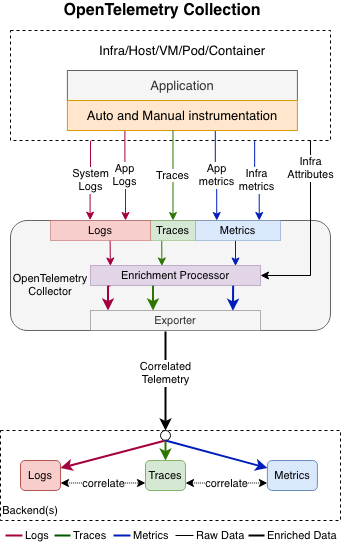
\includegraphics[width=\linewidth]{img/03_methoden/otel_unified-collection_2.png}
%	\caption{Schaubild einer Lösung auf Basis von OTel \cite{OpenTelemetryUnifiedCollection}}
%	\label{fig:otel-unified-collection}
%\end{figure}
%
%\begin{figure}[H]
%	\centering
%	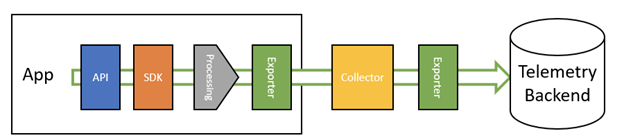
\includegraphics[width=0.75\linewidth]{img/03_methoden/dynatrace_otel-components.png}
%	\caption{OTel Komponenten \cite{DynatraceOTelComponents}}
%	\label{fig:otel-components}
%\end{figure}